\documentclass[11pt,a4paper]{article}
\usepackage[margin=24mm]{geometry}
\usepackage[T1]{fontenc}
\usepackage{lmodern,graphicx,booktabs,xcolor,hyperref}
\definecolor{signal}{HTML}{C84335}
\hypersetup{colorlinks=true,urlcolor=signal,linkcolor=signal,pdftitle={FUSE Multi-Repository Evaluation},pdfauthor={VIGIL}}
\newcommand{\ScannedFiles}{4347}
\newcommand{\SelectedFiles}{4348}
\newcommand{\RawFindings}{3}
\newcommand{\ScannerCommit}{93313780408799032b88462483a76ecbb641d2c1}
\newcommand{\ResultRows}{ArduPilot/ardupilot & 260/260 & 0 & complete \\
RT-Thread/rt-thread & 2126/2127 & 1 & partial \\
openbmc/openbmc & 230/230 & 0 & complete \\
meshtastic/firmware & 1731/1731 & 2 & partial \\}
\newcommand{\PinnedScopes}{\item ArduPilot/ardupilot: \texttt{278a68a57aa0d9b98e6dbaaf9346f6b485f4c9ac}. ArduCopter plus selected communications, networking, arming, HAL, and parameter libraries
\item RT-Thread/rt-thread: \texttt{cbc19778d0ae5ef2533a28c0f62c6a399858010a}. RTOS core, headers, networking, drivers, shell, utilities, and root configuration
\item openbmc/openbmc: \texttt{c9bb07fa438f008aa1c998fe2e742a386cd15776}. Phosphor service recipes and selected IBM host and network recipe extensions
\item meshtastic/firmware: \texttt{332b5b0a2c4fec2896de3c5fa63f46d5cd05ea98}. Firmware source, board variants, and selected build configuration}
\newcommand{\FindingItems}{\item RT-Thread/rt-thread: FUSE001, medium severity, high confidence. Credential-like literal in source Location: \texttt{components/finsh/shell.h}, line 47.
\item meshtastic/firmware: FUSE001, medium severity, high confidence. Credential-like literal in source Location: \texttt{src/mesh/Default.h}, line 79.
\item meshtastic/firmware: FUSE003, high severity, high confidence. TLS peer verification appears disabled Location: \texttt{src/mqtt/MQTT.cpp}, line 544.}
\newcommand{\MetadataLimits}{\item meshtastic/firmware: PlatformIO metadata contains unresolved interpolation; declared values are not effective build settings.}

\title{FUSE: Multi-Repository Static Inspection\\\large Coverage, Findings, and PlatformIO Refinement}
\author{A VIGIL Project}
\date{14 November 2026}
\begin{document}
\maketitle
\begin{abstract}
This exploratory regression replay evaluates the Firmware \& Unified Security Engine (FUSE) on four pinned source scopes spanning autopilot software, an RTOS, embedded Linux recipes, and radio firmware. FUSE scanned \ScannedFiles{} of \SelectedFiles{} selected files and emitted \RawFindings{} static review candidates. We report input coverage and configuration inventory separately from findings. This study evaluates selected scanner behavior; it does not establish vulnerability detection accuracy or deployed-device security.
\end{abstract}
\section{Research question and project selection}
Can FUSE preserve source findings while improving configuration inventory on varied embedded projects? We reuse the 12 November 2026 cohort to permit a direct regression comparison. The projects are selected for distinct engineering domains: \href{https://github.com/ArduPilot/ardupilot}{ArduPilot}, \href{https://github.com/RT-Thread/rt-thread}{RT-Thread}, \href{https://github.com/openbmc/openbmc}{OpenBMC}, and \href{https://github.com/meshtastic/firmware}{Meshtastic}. These scopes were previously inspected and informed refinement; this is a purposive regression set. It is not a fresh blind benchmark. Whole-repository security is outside the selected scopes.
\section{Method and provenance}
The manifest fixes upstream revisions, profiles, and include paths before scanning. The existing runner verifies clean pinned checkouts, hashes the FUSE source tree, runs native analysis offline, and preserves JSON, text, and SARIF output. It accepts incomplete scans only when the exit status agrees with report coverage. No target scripts, builds, or firmware execute. Syft, OSV-Scanner, Binwalk, Gitleaks, and Ghidra are disabled for this experiment. One run per scope provides functional evidence; no performance comparison or statistical inference is attempted.

Scanner version: 0.3.0, development source commit \texttt{\ScannerCommit}. This refinement is newer than the published 0.3.0 distribution. Environment: Windows, Python 3.14. Matplotlib 3.10.8 generates the figures from preserved reports. The manifest records the scanner source digest; metrics.json records each input report digest.
\begin{itemize}\PinnedScopes\end{itemize}
\section{Implemented refinement}
The prior resolver handled one environment parent and missed common sections and multiple parents. The configuration file limit also rejected a Meshtastic pattern containing 185 files. The revised reader resolves literal section references, applies later-parent and child overrides, handles multiline defaults and inline comments, and supports up to 512 configuration files. Existing per-file and total-byte caps remain, with an additional inheritance-depth cap of 32. Reported interpolation remains declared text and causes partial status. No host environment variables or project scripts are evaluated.

The semantics follow the upstream \href{https://docs.platformio.org/en/latest/projectconf/sections/env/options/advanced/extends.html}{PlatformIO inheritance documentation} and \href{https://docs.platformio.org/en/latest/projectconf/sections/platformio/options/generic/extra_configs.html}{extra configuration documentation}. Regression controls cover parent precedence, environment defaults, cycles, unresolved variables, and a 200-environment matrix. The full local suite passed 354 tests and 157 subtests, with one skipped test. Hosted cross-platform checks are separate evidence.
\section{Results}
\begin{center}\begin{tabular}{lrrl}\toprule
Project & Scanned/selected & Findings & Coverage\\\midrule
\ResultRows
\bottomrule\end{tabular}\end{center}
\begin{figure}[htbp]\centering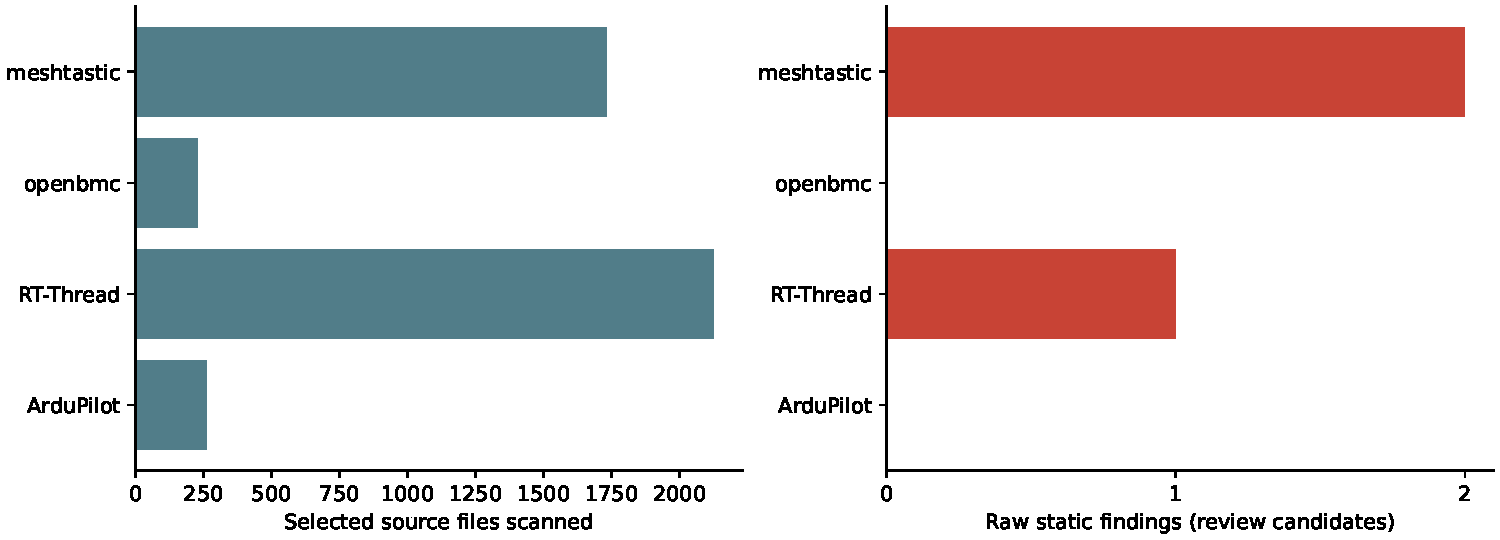
\includegraphics[width=\linewidth]{scan-results.pdf}\caption{Source-file counts and raw static signals for the selected scopes. Count differences reflect scope and project size, not security rankings.}\end{figure}
\begin{figure}[htbp]\centering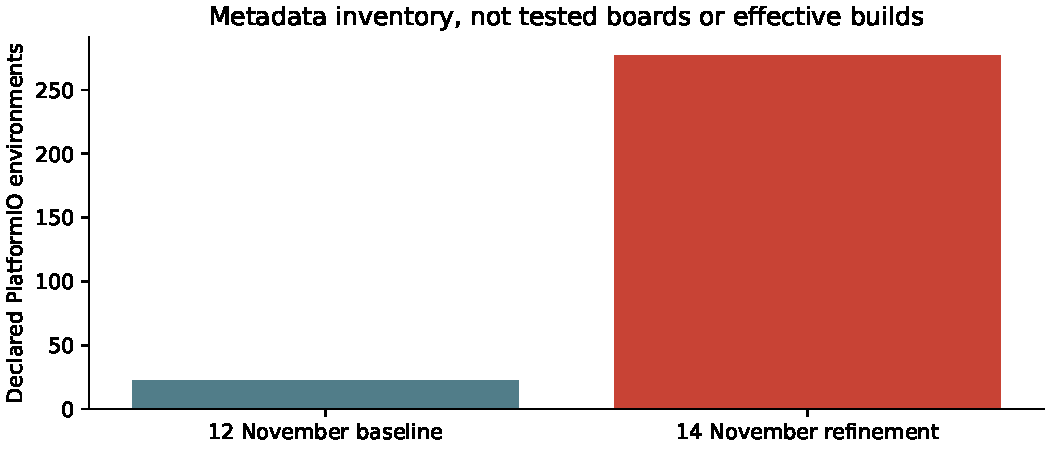
\includegraphics[width=.82\linewidth]{platformio-context.pdf}\caption{Declared environment inventory before and after refinement. Environments are configuration declarations; no boards were built or tested.}\end{figure}
\subsection{Review candidates}
\begin{itemize}\FindingItems\end{itemize}
Severity expresses potential impact and confidence expresses strength of static evidence. The earlier source review identified password-like defaults and a conditional TLS-verification bypass. This replay does not add an independent adjudicator or validate reachability. Findings retain candidate status. Zero findings means no enabled rule matched the selected inputs.
\subsection{Incomplete coverage}
RT-Thread contains a selected file exceeding the source-size cap. The file remains skipped and the scope remains partial. PlatformIO metadata limitations are reproduced below rather than hidden by the increased environment count.
\begin{itemize}\MetadataLimits\end{itemize}
\section{Threats to validity and next steps}
Selection is purposive and scopes are limited. Prior exposure makes tuning leakage possible. Shared Windows execution does not prove portability to all systems. Native rules inspect a narrow set of source patterns; absent vulnerability ground truth prevents precision, recall, or missed-vulnerability estimates. Static defaults and conditional code do not establish shipped-device exposure. Input hashes improve reproducibility but do not authenticate upstream provenance.

The next universality steps are compiler-aware source analysis using selected compilation databases, independent labeled vulnerable and secure controls across frameworks, and build-configuration evidence for additional platforms. Imported analyzer evidence should retain its tool version, source scope, limits, and confidence. A broader feature list alone cannot establish industry readiness.
\section{Reproduction and publication}
The cohort README provides scanner and publication commands. Rebuild figures and generated tables using scripts/build\_multi\_repository\_report.py, then compile this document twice with pdflatex using shell escape disabled. The repository report workflow installs the pinned plotting dependency, builds the PDF, uploads the publication directory as a Pages artifact, and deploys only from main. Pull requests build for review without deployment.
\end{document}
